\begin{figure}[!t]
    \centering
    \captionsetup[subfigure]{justification=centering,singlelinecheck=false}
    \newsavebox{\ipregretpanel}
    \sbox{\ipregretpanel}{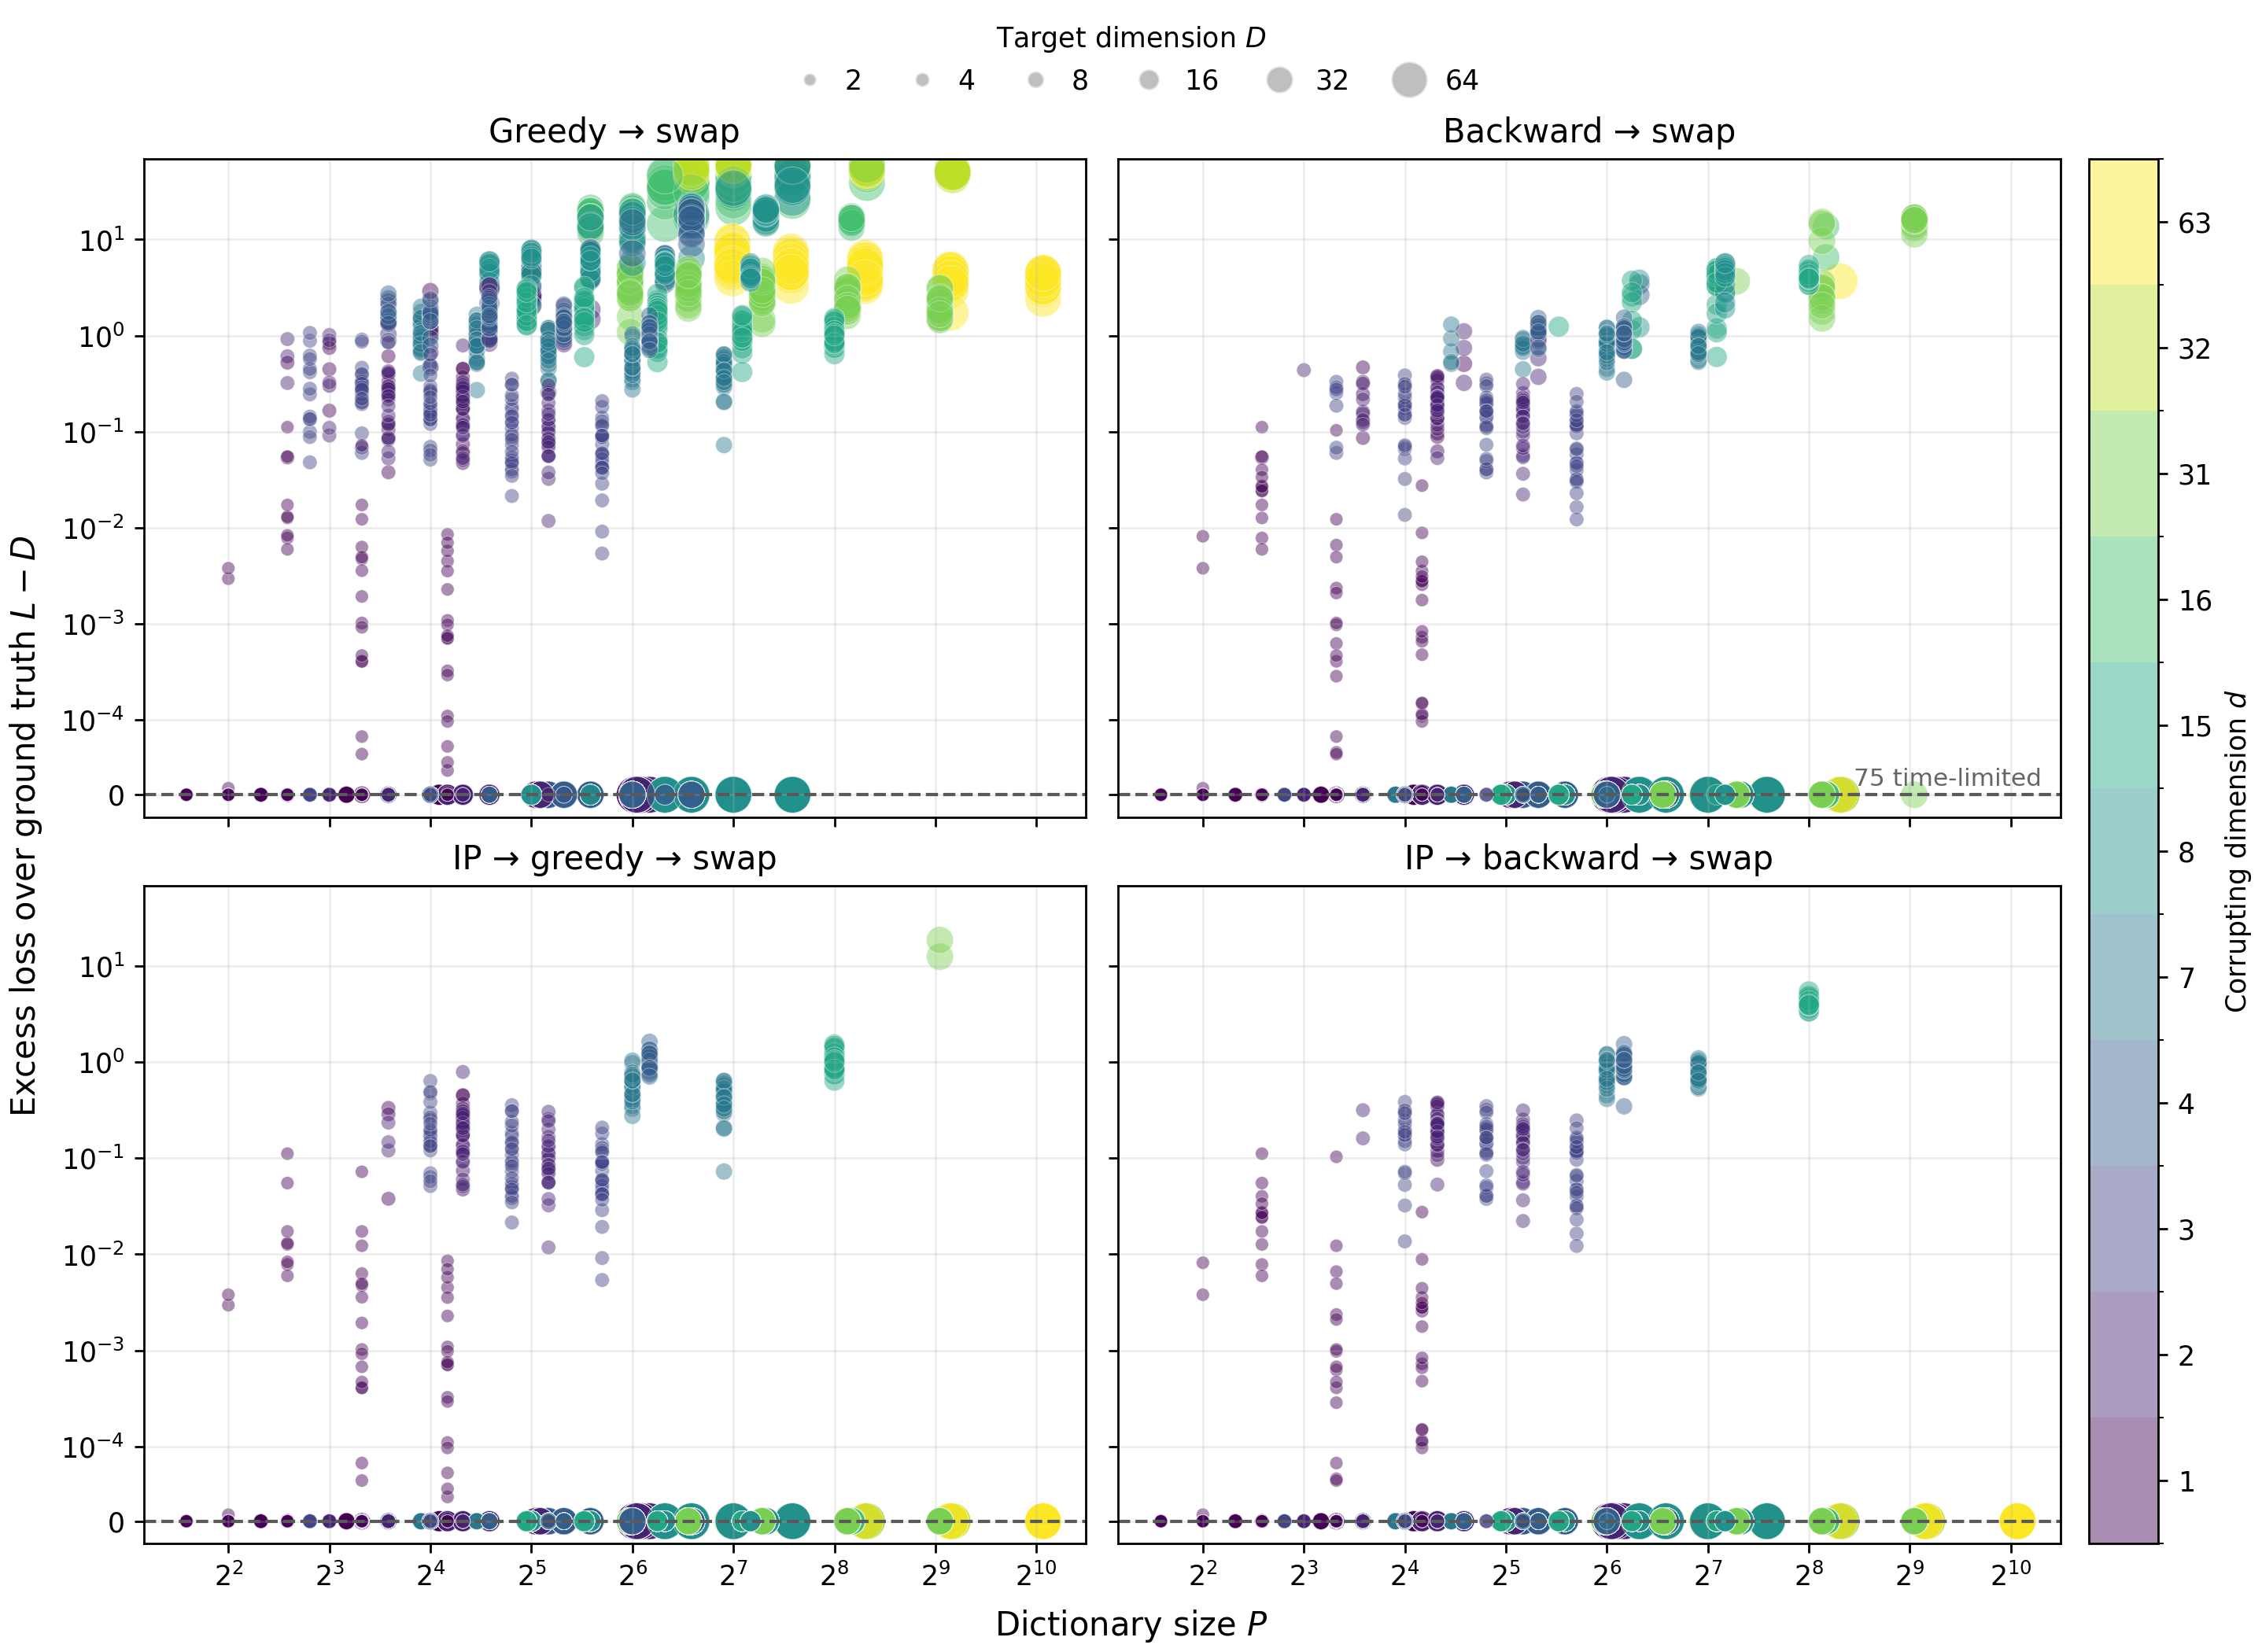
\includegraphics[width=0.36\textwidth]{../figures/synthetic_excess_loss_vs_dictionary.png}}
    \begin{subfigure}[t]{0.24\textwidth}
        \centering
        \begin{minipage}[c][\dimexpr\ht\ipregretpanel+\dp\ipregretpanel\relax][c]{\linewidth}
            \centering
            \resizebox{\linewidth}{!}{%
            \begin{tabular}{lrrr}
                \toprule
                Dataset & $D$ & $P$ & $R$ \\
                \midrule
                Synthetic & $2$--$64$ & $3$--$1072$ & $25$ \\
                Iris & $4$ & $75$ & $25$ \\
                Wine & $13$ & $89$ & $25$ \\
                Ethanol & $2$ & $756$ & $25$ \\
                \bottomrule
            \end{tabular}}
            \par\smallskip
            {\scriptsize $R$ is per synthetic condition.}
        \end{minipage}
        \caption{Dataset parameters.}
        \label{fig:experiment-datasets}
    \end{subfigure}\hfill
    \begin{subfigure}[t]{0.36\textwidth}
        \centering
        \begin{minipage}[c][\dimexpr\ht\ipregretpanel+\dp\ipregretpanel\relax][c]{\linewidth}
            \centering
            \usebox{\ipregretpanel}
        \end{minipage}
        \caption{Synthetic ground-truth regret.}
        \label{fig:synthetic-ground-truth-regret}
    \end{subfigure}\hfill
    \begin{subfigure}[t]{0.36\textwidth}
        \centering
        \begin{minipage}[c][\dimexpr\ht\ipregretpanel+\dp\ipregretpanel\relax][c]{\linewidth}
            \centering
            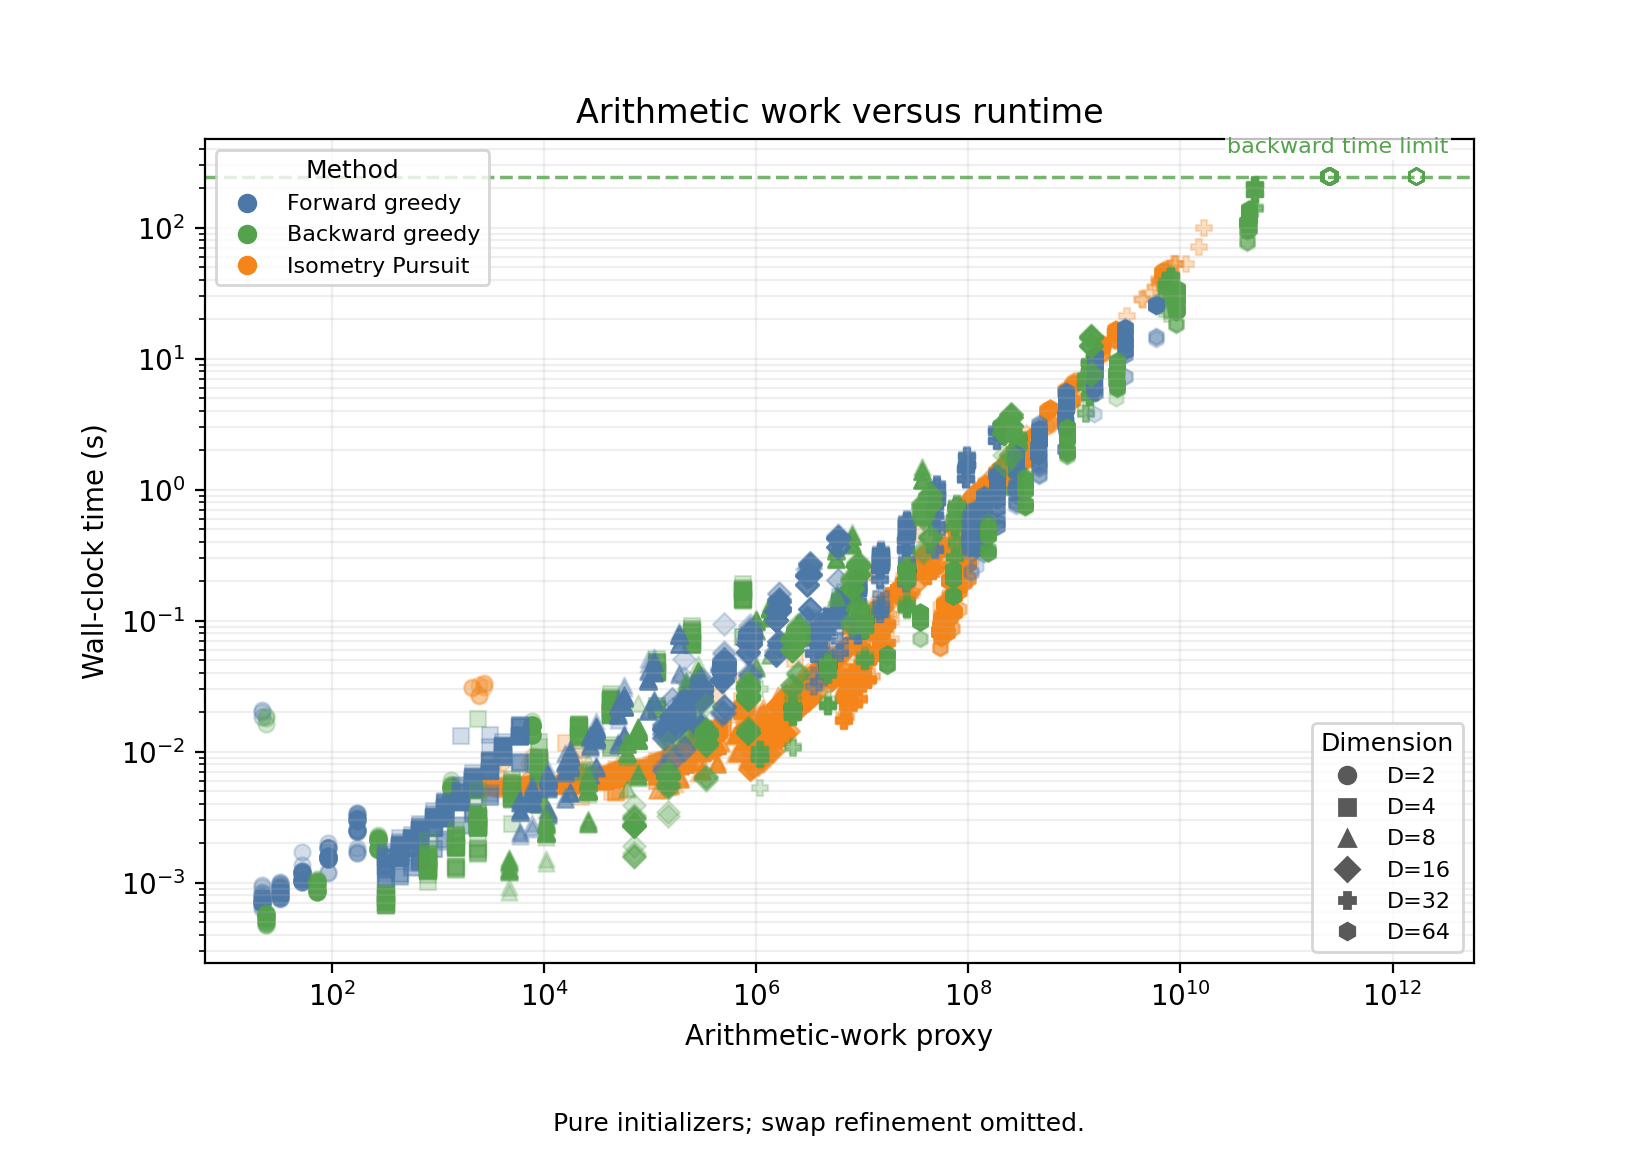
\includegraphics[width=\linewidth]{../figures/complexity_runtime/complexity_vs_runtime_main.png}
        \end{minipage}
        \caption{Arithmetic work versus runtime.}
        \label{fig:complexity-runtime-early-stop}
    \end{subfigure}
    \par\medskip
    \begin{subfigure}[t]{\textwidth}
        \centering
        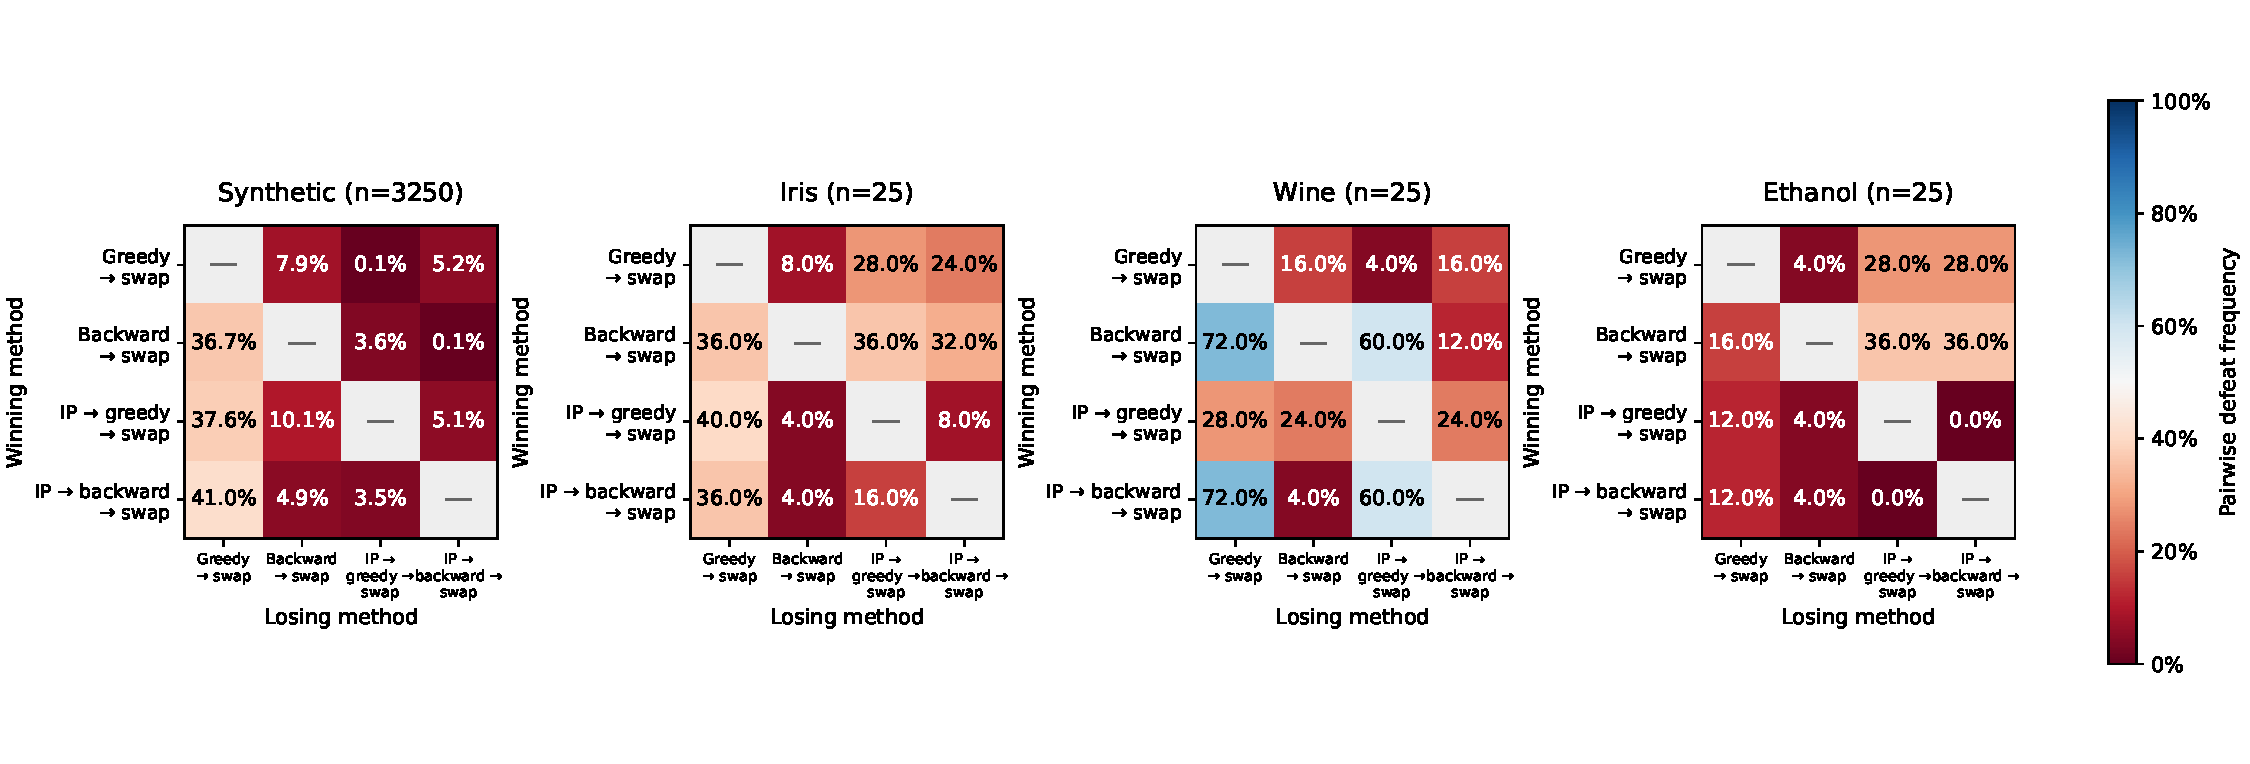
\includegraphics[width=\linewidth]{../figures/optimizer_defeats/optimizer_defeat_matrices.pdf}
        \caption{Pairwise defeat frequencies.}
        \label{fig:real-search-regrets}
    \end{subfigure}
\caption{Statistical and computational behavior of the four search pipelines.
(a) Dataset parameters.
(b,c) The same $3250$ fixed synthetic matrices cover $130$ conditions at $D=2,4,8,16,32,64$, with $25$ replicates per condition and IP using SCS at scale $0.1$.
(b) Final-search regret relative to the raw-loss optimum $D$; text reports time-limited pipelines.
(c) Arithmetic-work proxies versus Lambda runtime for pure initializers, excluding swaps.
Open markers indicate backward initializers reaching the $245$-second limit (dashed line), plotted against full-elimination work.
(d) Strict pairwise defeat frequencies for Synthetic, Iris, Wine, and Ethanol, each with $25$ replicates per condition or real dataset.
Each cell uses only runs where both searches completed, so denominators vary when searches timed out; ties earn no win credit.}
\end{figure}
